\section{Krav til dynamikken}

I dette afsnit beskrives kravene til hvilken funktionalitet systemet har. Der er opstillet følgende række krav i første omgang.
\begin{itemize}
	\item Systemet kan regulere en horisontal vinkel på op til ±30 grader tilbage til vandret i ”overdelen”
	\item Overshoot max 5\%
	\item Settlingtime 0.5 sekund 
	\item Stationær fejl max 10\%  
	
\end{itemize}



Herunder i \autoref{fig:Blokdiagram} vises et blokdiagram, som viser en beskrivelse af systemets (fysiske) blokke, som beskriver opbygningen af systemet på Lego bilens styringsenhed. 


\begin{figure}[H]
	\centering
	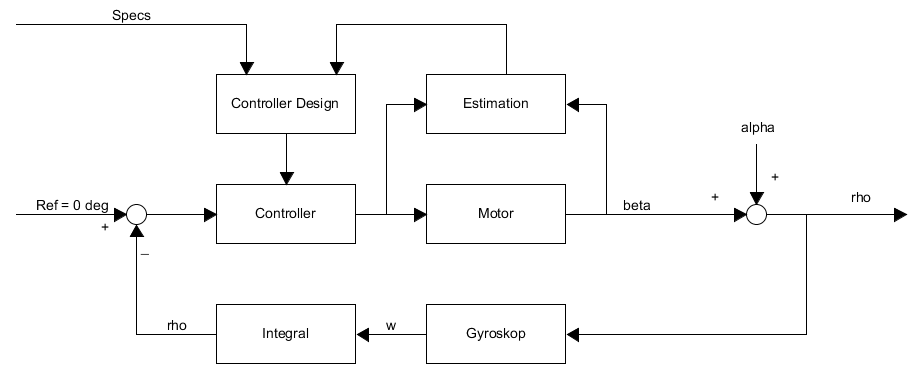
\includegraphics[width = 400 pt]{figur/blokdiagram.png}
	\caption{Blokdiagram}
	\label{fig:Blokdiagram}
\end{figure}

\textit{beta} er motorens vinkel,\textit{ alpha} er vinkel forstyrrelsen fra terrænets hældning. \textit{rho} er vinkelen på selve overdelen af Lego bilen. Det er denne vinkel \textit{rho}, som gerne forsøges at reguleres til 0 grader eller vandret. Outputtet fra gyroskopet er en vinkelhastighed som igennem integration laves om til en vinkel ændring i forhold til start vinklen (helst vandret). Controlleren er tænkt som en pol placerings regulator, men som i første omgang ikke er adaptiv ved brug parameter estimation af modellen (MIAC). 